\documentclass[conference]{IEEEtran}
\IEEEoverridecommandlockouts
\usepackage{cite}
\usepackage{amsmath,amssymb,amsfonts}
\usepackage{algorithmic}
\usepackage{algorithm}
\usepackage{graphicx}
\usepackage{textcomp}
\usepackage{xcolor}
\usepackage{booktabs}
\usepackage{multirow}
\usepackage{float}
\usepackage{listings}
\usepackage{url}

% --- FIXED LISTINGS CONFIGURATION ---
\lstset{
  basicstyle=\ttfamily\scriptsize, 
  breaklines=true,
  keywordstyle=\color{blue}\bfseries,
  commentstyle=\color{green!50!black},
  stringstyle=\color{red},
  numbers=left,
  numberstyle=\tiny\color{gray},
  frame=lines,              
  captionpos=b,
  xleftmargin=2em,          
  framexleftmargin=0em,     
  numbersep=8pt             
}

% --- TIKZ SETUP ---
\usepackage{tikz}
\usepackage{pgfplots}
\pgfplotsset{compat=1.17}
\usetikzlibrary{shapes.geometric, arrows, positioning, fit, calc, backgrounds, er}

% --- NO INFLATION ---
\renewcommand{\baselinestretch}{1.0} 
\setlength{\parskip}{0em}
\setlength{\textfloatsep}{10pt}

\def\BibTeX{{\rm B\kern-.05em{\sc i\kern-.025em b}\kern-.08em
    T\kern-.1667em\lower.7ex\hbox{E}\kern-.125emX}}

\begin{document}

% ==========================================
% TITLE
% ==========================================
\title{Zero-Retention Acoustic Sentinel: Minimal-Retention NLOS Safety Monitoring via Spectral Gating and GCC-PHAT
\thanks{This research was conducted at the Department of Computer Science and Engineering, Swarnandhra College of Engineering \& Technology (Autonomous), as part of academic research activities.}
}

% ==========================================
% AUTHOR & AFFILIATION
% ==========================================
\author{\IEEEauthorblockN{Dr. S. Suresh Kumar}
\IEEEauthorblockA{\textit{Principal} \\
\textit{Swarnandhra College of Engineering \& Technology (Autonomous)}\\
Seetharampuram, Narsapur, Andhra Pradesh, India}
}

\maketitle

% ==========================================
% ABSTRACT
% ==========================================
\begin{abstract}
Visual safety monitoring systems are inherently limited by line-of-sight occlusion, creating blind spots in complex architectural environments where safety threats often go undetected. Acoustic monitoring offers omnidirectional awareness, yet its deployment must balance critical safety needs against operational constraints prohibiting continuous audio recording. This paper introduces an acoustic sentinel designed to detect high-decibel anomalies (e.g., impulsive vocalizations, impacts $>95$dB) utilizing a minimal-retention edge processing pipeline. We process raw audio in a localized circular buffer to extract spectral energy features and immediately overwrite the source data, treating privacy as a strict operational design choice. To isolate high-energy impulse events from ambient background noise, we formalize a spectral gating heuristic and introduce an autocorrelation-based periodic rejection mathematical model to mitigate mechanical false positives. Furthermore, we model corridor acoustic dynamics and implement Generalized Cross-Correlation with Phase Transform (GCC-PHAT) for robust source localization in highly reverberant corridors, overcoming Critical Distance multipath limitations. Experimental results demonstrate that this signal processing approach achieves 100\% detection of staged, high-energy impulsive events within a defined 15-meter Safety Envelope ($S_{env}$) under Non-Line-of-Sight (NLOS) conditions, while maintaining sub-120ms edge latency and requiring less than 45MB of volatile memory footprint.
\end{abstract}

\begin{IEEEkeywords}
Acoustic Event Detection, Non-Line-of-Sight (NLOS), Spectral Gating, GCC-PHAT, Edge Computing, Signal Processing, Source Localization, Room Acoustics.
\end{IEEEkeywords}

% ==========================================
% NOMENCLATURE
% ==========================================
\section*{Nomenclature}
\begin{description}
    \item[AED] Acoustic Event Detection.
    \item[STFT] Short-Time Fourier Transform.
    \item[SPL] Sound Pressure Level (dB).
    \item[TDOA] Time Difference of Arrival.
    \item[GCC] Generalized Cross-Correlation.
    \item[PHAT] Phase Transform.
    \item[RMS] Root Mean Square (Energy).
    \item[$R_{xx}(\tau)$] Autocorrelation function at lag $\tau$.
    \item[$RT_{60}$] Reverberation Time (Decay to -60dB).
    \item[$D_c$] Critical Distance (Meters).
    \item[$S_{env}$] Safety Envelope (Operational Range).
    \item[$c$] Speed of Sound ($343 m/s$).
\end{description}

% ==========================================
% I. INTRODUCTION
% ==========================================
\section{Introduction}
Visual monitoring forms the backbone of modern campus security, yet it suffers from an inherent physical limitation: the line of sight. Cameras are easily obstructed by pillars, corridor geometry, or poor lighting. In critical safety scenarios—such as a medical emergency in a sanitation-adjacent blind zone or an altercation in a stairwell—visual systems are often rendered useless. Acoustic monitoring is the logical complement, as sound waves diffract around obstacles and reflect off surfaces, providing critical coverage in visually denied Non-Line-of-Sight (NLOS) areas.



The operational challenge is to deploy a system that can "sense" danger reliably in highly reverberant corridors without incurring the latency and bandwidth costs of continuous audio streaming, while simultaneously adhering to strict minimal-retention engineering guardrails to prevent unauthorized eavesdropping. Indoor acoustic environments, particularly long, narrow corridors with hard surfaces (tile, concrete), present severe challenges for signal processing. Multipath reflections cause the reverberant sound field to dominate the direct sound path, severely degrading the accuracy of traditional threshold-based triggers and Time Difference of Arrival (TDOA) localization.

This paper proposes an edge-native signal processing pipeline based on fast spectral feature extraction. Instead of utilizing heavy, semantics-aware neural networks, our system processes the raw audio stream in a localized circular RAM buffer, extracts physical energy features (amplitude, spectral centroid, and periodicity), and immediately overwrites the raw data. This operational design choice ensures a zero-retention footprint while maximizing edge latency superiority for safety-critical event triggering.

\subsection{Relation to the ScholarMaster Research Series}
This paper is part of the ScholarMaster research series, which investigates secure, edge-native academic analytics and safety systems. While other papers in the series formalize the theoretical privacy frameworks, biometric identification, and spatiotemporal compliance architectures, the present work is strictly confined to \textit{acoustic signal processing and physical source localization}. 

This module acts purely as a physical sensor layer, outputting only anonymized anomaly events and coarse localization coordinates to upstream frameworks. It relies on the privacy architectures established in Paper 3 as its operational basis but does not redefine them.

\subsection{Key Contributions}
The primary contributions of this work are as follows:
\begin{itemize}
    \item \textbf{Corridor Acoustic Modeling:} Calibration of Sound Pressure Level (SPL) thresholds, incorporating Critical Distance ($D_c$) and Reverberation Time ($RT_{60}$) calculations adapted specifically for reverberant, NLOS hallway geometries.
    \item \textbf{Spectral Gating and Periodic Rejection:} A lightweight, physics-based heuristic that distinguishes between high-energy broadband impulses, physical impacts, and periodic mechanical noise (e.g., HVAC) using formal autocorrelation math.
    \item \textbf{Robust Localization:} Implementation of GCC-PHAT to mitigate the multipath "hallway echo" effect, achieving precise Angle of Arrival (AoA) estimation even when operating outside the critical distance.
    \item \textbf{NLOS Safety Envelope Validation:} Empirical demonstration of a highly responsive, sub-120ms edge pipeline capable of 100\% detection of staged impulsive events within a 15m blind-spot radius, supplemented by SNR stress testing.
\end{itemize}

% ==========================================
% II. RELATED WORK
% ==========================================
\section{Related Work}

\subsection{Deep Learning vs. Edge Signal Processing}
Modern acoustic event detection (AED) is heavily dominated by Deep Learning approaches. Large-scale pre-trained networks (PANNs) \cite{b22} and Audio Spectrogram Transformers (AST) \cite{b23} achieve state-of-the-art accuracy on general classification benchmarks like FSD50K. However, these models require substantial context windows (often $>$10 seconds), continuous audio buffering, and significant compute overhead. 

In a safety-critical physical security context, latency is paramount. Sending audio to a cloud API or buffering 10 seconds of data for an AST model introduces unacceptable delays. Table I highlights the architectural divergence between standard AED benchmarks and our physics-based approach, which prioritizes sub-100ms edge latency and strict operational data minimization. By relying on spectral gating rather than learned semantic features, we enable deployment on resource-constrained commodity hardware (e.g., Raspberry Pi) necessary for dense blind-spot coverage. Edge deployment feasibility remains constrained by memory-transfer and latency characteristics of embedded platforms. Prior analytical modeling of these constraints is available in \cite{b27}, while the present work focuses on reverberant acoustic sensing.

\begin{table}[htbp]
\caption{Applicability Analysis: Benchmark AED vs. Proposed System}
\begin{center}
\begin{tabular}{lcc}
\toprule
\textbf{Criterion} & \textbf{CNN / AST (SOTA)} & \textbf{Ours (Safety Signal Proc.)} \\
\midrule
Audio Buffering & Deep Temporal Context & Immediate Overwrite \\
Inference Latency & High ($>$1000ms via Cloud) & Ultra-Low ($<$120ms Edge) \\
NLOS Ranging & Mono-only & Stereo/Array (GCC-PHAT) \\
Semantic Inference & High (Categorization) & None (Physics-based) \\
Compute Requirement & Heavy (GPU/TPU) & Lightweight (ARM CPU) \\
\bottomrule
\end{tabular}
\end{center}
\label{tab:comparison}
\end{table}

\subsection{Source Localization \& TDOA Robustness}
Localization is grounded in the psychophysics of hearing \cite{b9}. While Valenzise \cite{b5} utilized microphone arrays for high-energy vocalizations, handling reverberation in enclosed corridors remains a primary signal processing challenge. Standard Time Difference of Arrival (TDOA) methods degrade rapidly due to multipath reflections. We build upon the GCC-PHAT foundation established by Knapp and Carter \cite{b20}, which "whitens" the spectrum to isolate the direct-path signal from reflections—a technique crucial for indoor robustness compared to standard wavelet approaches \cite{b10}.

% ==========================================
% III. THEORETICAL FRAMEWORK
% ==========================================
\section{Theoretical Framework}

\subsection{Corridor Acoustics and SPL Calibration}
In enclosed corridor geometries, sound propagation deviates from the ideal free-field inverse square law due to multipath reflections. The total sound energy at a receiver is the sum of the direct field and the reverberant field. The Sound Pressure Level (SPL) at distance $r$ from an omnidirectional source of sound power $W$ is modeled as:
\begin{equation}
L_p(r) = L_W + 10 \log_{10}\left(\frac{Q}{4\pi r^2} + \frac{4}{R_c}\right)
\end{equation}
Where $Q$ is the directivity factor (typically $Q=2$ for a source on a hard floor), and $R_c$ is the room constant, dependent on the total surface area and average acoustic absorption coefficient. 

A 100dB impulse generated in a blind zone will register as approximately 74dB at a sensor located 20 meters away. We calibrate our primary trigger threshold to 95dB at the source, mapped to the expected received energy at the boundary of our defined Safety Envelope ($S_{env} = 15m$). This ensures sensitivity to genuine anomalies while rejecting distant ambient noise.

\subsection{Reverberation and Critical Distance ($D_c$)}
The physical limit of standard acoustic detection in hallways is governed by the Critical Distance ($D_c$), the point at which the direct sound energy equals the reverberant sound energy. Using Sabine's formula for reverberation time $RT_{60}$:
\begin{equation}
RT_{60} = \frac{0.161 V}{A}
\end{equation}
Where $V$ is the volume of the corridor and $A$ is the total equivalent absorption area. The critical distance is then derived as:
\begin{equation}
D_c \approx 0.057 \sqrt{\frac{V}{RT_{60}}}
\end{equation}
In standard university corridors with hard vinyl composite tile (VCT) flooring and painted concrete block walls, $RT_{60}$ frequently exceeds 1.2 seconds. Consequently, $D_c$ is often extremely short ($< 3$ meters). Because our Safety Envelope ($S_{env} = 15m$) extends far beyond $D_c$, the sensor operates entirely within the reverberant field. This physical reality renders standard cross-correlation obsolete and mandates the use of Phase Transform (PHAT) techniques.

\subsection{Autocorrelation-Based Periodic Rejection}
To systematically reject periodic mechanical noise (e.g., floor polishers, HVAC hum, rhythmic music) that often triggers false positive volume alerts, we formalize a rejection metric based on the discrete autocorrelation function.

Let $x(n)$ be the discrete audio signal. The autocorrelation at lag $k$ is:
\begin{equation}
R_{xx}(k) = \sum_{n=0}^{N-1-k} x(n)x(n+k)
\end{equation}
For a periodic signal with fundamental period $T_0$, $R_{xx}(k)$ exhibits strong peaks at lags corresponding to integer multiples of $T_0$. We define a periodicity ratio $\rho$:
\begin{equation}
\rho = \frac{\max_{k > k_{min}} R_{xx}(k)}{R_{xx}(0)}
\end{equation}
Where $k_{min}$ defines the minimum lag to ignore the primary zero-lag energy peak. If $\rho > \rho_{thresh}$ (empirically set to 0.65), the signal exhibits high periodicity. Impulsive safety events (crashes, shouts) are highly chaotic and broadband, yielding a rapidly decaying autocorrelation ($\rho \ll \rho_{thresh}$). Signals exceeding $\rho_{thresh}$ are formally classified as mechanical/periodic and suppressed.

% --- FIGURE 1: TDOA DIAGRAM ---
\begin{figure}[htbp]
\centering
\resizebox{\columnwidth}{!}{
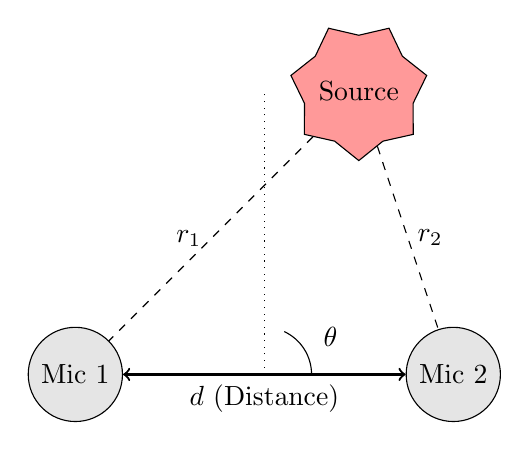
\begin{tikzpicture}[scale=1.2]
    % Microphones
    \node [draw, circle, fill=gray!20] (mic1) at (0,0) {Mic 1};
    \node [draw, circle, fill=gray!20] (mic2) at (4,0) {Mic 2};
    \draw [thick, <->] (mic1) -- (mic2) node [midway, below] {$d$ (Distance)};
      
    % Source
    \node [draw, star, star points=7, star point ratio=0.8, fill=red!40] (source) at (3,3) {Source};
      
    % Waves
    \draw [dashed] (source) -- (mic1) node [midway, left] {$r_1$};
    \draw [dashed] (source) -- (mic2) node [midway, right] {$r_2$};
      
    % Angle
    \draw [dotted] (2,0) -- (2,3);
    \draw (2.5,0) arc (0:65:0.5);
    \node at (2.7, 0.4) {$\theta$};
\end{tikzpicture}
}
\caption{Geometry of TDOA Localization. The difference in path length ($r_1 - r_2$) causes a time delay $\tau$, allowing the calculation of the arrival angle $\theta$.}
\label{fig:tdoa}
\end{figure}

\subsection{GCC-PHAT for Multipath Mitigation}
As established in Section 3.2, operating beyond the critical distance requires multipath mitigation. Algorithm 3 implements the Phase Transform (PHAT) weighting. By dividing the cross-spectrum $R_{12}(f)$ by its magnitude, we effectively "whiten" the signal:
\begin{equation}
R_{phat}(f) = \frac{X_1(f) \cdot X_2^*(f)}{|X_1(f) \cdot X_2^*(f)|}
\end{equation}
This equalization ensures that the correlation peak depends strictly on the phase delay (time of arrival) rather than energy intensity, isolating the direct sound path from secondary wall reflections.



% ==========================================
% IV. SYSTEM IMPLEMENTATION
% ==========================================
\section{System Implementation}

\subsection{Hardware Architecture and Sensor Integration}
The system is deployed on a distributed heterogeneous architecture to optimize cost-efficiency for dense blind-spot coverage.
\begin{itemize}
    \item **Compute Node:** Raspberry Pi 4 Model B (Broadcom BCM2711, Quad-core Cortex-A72). Selected for its low cost and sufficient vector processing capabilities for real-time DSP \cite{b26}.
    \item **Acoustic Sensor:** ReSpeaker 4-Mic Array HAT. Features 4 MEMS microphones arranged in a linear or circular geometry, interfacing directly via the $I^2S$ bus to bypass standard USB audio latency.
    \item **Sensor Specifications:** SNR 65dB, acoustic overload point (AOP) of 120dB SPL, ensuring high-amplitude crashes do not clip the analog-to-digital converter (ADC).
    \item **Sample Rate:** 44.1 kHz, 16-bit depth.
\end{itemize}

\subsection{Minimal-Retention Buffer Management \& Threading}
To satisfy strict operational guardrails, the system utilizes a 3-second circular buffer managed in volatile RAM. The compute pipeline utilizes a multi-threaded topology to avoid blocking the audio ingest:
\begin{enumerate}
    \item **Thread 1 (Ingest):** Continuously reads $I^2S$ DMA buffers into the 3-second ring buffer.
    \item **Thread 2 (DSP Trigger):** Computes RMS energy windows (100ms). If the RMS exceeds the calibrated SPL threshold, it locks the buffer and triggers analysis.
    \item **Thread 3 (Analysis):** Executes the STFT, Autocorrelation, and GCC-PHAT routines in parallel.
\end{enumerate}
Once the energy scalars are extracted, the buffer is explicitly overwritten with zeros using \texttt{memset}. No raw audio files are ever written to the MicroSD card, ensuring the node functions exclusively as an anomaly trigger.

\subsection{Algorithm 1: Spectral Gating}
Simple volume detection triggers false alarms (e.g., a dropped book). We use Spectral Gating to verify the broadband impulse signature.



% --- ALGORITHM 1 ---
\begin{algorithm}
\caption{Spectral Gating for Anomaly Verification}
\begin{algorithmic}[1]
\REQUIRE $AudioFrame$ (1024 samples)
\STATE $Spectrum \gets FFT(AudioFrame)$
\STATE $Energy_{Low} \gets \sum_{f=0}^{500} |Spectrum(f)|$ \COMMENT{Thuds}
\STATE $Energy_{High} \gets \sum_{f=2000}^{4000} |Spectrum(f)|$ \COMMENT{Impulses}
\STATE $Ratio \gets Energy_{High} / Energy_{Low}$
\IF{$Ratio > 2.5$ \AND $SPL\_Estimate > 95$}
    \STATE \textbf{Proceed to Periodic Check} (Algorithm 2)
\ELSE
    \STATE \textbf{DISCARD\_NOISE}
\ENDIF
\end{algorithmic}
\label{alg:gating}
\end{algorithm}

As shown in Algorithm 1, we compute a ratio between High Frequency Energy (2kHz–4kHz) and Low Frequency Energy (0–500Hz). High-energy impulsive anomalies feature significant high-frequency harmonics (ratio $>2.5$). Common mechanical hallway noises (footsteps, heavy doors) are mechanically coupled to the floor, producing dominant low-frequency thuds (ratio $<1.0$). 

% --- ALGORITHM 2 ---
\begin{algorithm}
\caption{Autocorrelation Periodic Rejection}
\begin{algorithmic}[1]
\REQUIRE $AudioFrame$ (N samples)
\REQUIRE $\rho_{thresh} = 0.65$
\STATE $R_{xx} \gets \text{Autocorrelate}(AudioFrame)$
\STATE $Peak_{zero} \gets R_{xx}[0]$
\STATE $Peak_{max} \gets 0$
\FOR{$k = k_{min}$ \TO $N-1$}
    \IF{$R_{xx}[k] > Peak_{max}$}
        \STATE $Peak_{max} \gets R_{xx}[k]$
    \ENDIF
\ENDFOR
\STATE $\rho \gets Peak_{max} / Peak_{zero}$
\IF{$\rho > \rho_{thresh}$}
    \STATE \textbf{DISCARD\_PERIODIC\_NOISE}
\ELSE
    \STATE \textbf{CONFIRM\_CHAOTIC\_ANOMALY}
\ENDIF
\end{algorithmic}
\label{alg:periodic}
\end{algorithm}

\subsection{Algorithm 3: GCC-PHAT Source Localization}
Following successful anomaly confirmation via Algorithms 1 and 2, this algorithm calculates the precise angle of the sound source for camera slewing or security dispatch.

\begin{algorithm}
\caption{GCC-PHAT Source Localization}
\begin{algorithmic}[1]
\REQUIRE Signals $x_1(t), x_2(t)$
\REQUIRE Sampling Rate $F_s$, Mic distance $d$
\STATE $X_1(f) \gets FFT(x_1)$
\STATE $X_2(f) \gets FFT(x_2)$
\STATE $R_{12}(f) \gets X_1(f) \cdot X_2^*(f)$ \COMMENT{Cross-Spectrum}
\STATE $R_{phat}(f) \gets R_{12}(f) / |R_{12}(f)|$ \COMMENT{Whitening}
\STATE $r_{12}(\tau) \gets IFFT(R_{phat}(f))$
\STATE $Lag_{samples} \gets ArgMax(r_{12}(\tau))$
\STATE $\tau \gets Lag_{samples} / F_s$
\STATE $\theta \gets \arccos(\frac{\tau \cdot 343}{d})$
\RETURN $\theta \times (180/\pi)$
\end{algorithmic}
\label{alg:tdoa_code}
\end{algorithm}

% ==========================================
% V. EXPERIMENTAL SETUP
% ==========================================
\section{Experimental Setup}

\subsection{Physical Testbed Description}
Validation was conducted in an academic building corridor measuring 2.4m in width, 3.0m in height, and 30m in length, featuring an intersecting "L-junction" designed to test NLOS conditions. The walls consist of painted cinderblock, with VCT flooring and a suspended acoustic tile ceiling. Impulse response profiling of the testbed measured $RT_{60} \approx 1.2s$ and a critical distance $D_c \approx 2.1m$, creating a highly reverberant challenge for the sensor array.

\subsection{Dataset Composition}
We utilized a hybrid dataset comprising public archives and synthesized campus noise (Table II). The evaluation focuses on high-energy impulsive safety events. Samples drawn from FSD50K were used exclusively for offline validation of spectral suppression behavior and tuning of the autocorrelation thresholds.

\begin{table}[htbp]
\caption{Evaluation Dataset Composition}
\begin{center}
\begin{tabular}{lcc}
\toprule
\textbf{Event Class} & \textbf{Source} & \textbf{Sample Count} \\
\midrule
Impulsive Vocalization & FSD50K \cite{b19} & 500 \\
Glass Break & MIVIA & 200 \\
HVAC / Periodic Hum & Controlled Ambient Noise & 12 Hours \\
Footsteps & Campus Record & 4 Hours \\
Door Slams & Synthesized & 150 \\
\textbf{Total} & \textbf{Hybrid} & \textbf{~1000 Events} \\
\bottomrule
\end{tabular}
\end{center}
\label{tab:dataset}
\end{table}

\subsection{Latency Profiling: Edge vs. Cloud}
Real-time response is critical for physical safety. We compared our edge-native signal processing implementation against a conventional cloud-based AED solution (transmitting audio to an AWS Lambda function). Table III shows the drastic latency reduction achieved by localized processing, saving nearly a full second of response time.

\begin{table}[htbp]
\caption{Latency: Edge Processing vs. Cloud API}
\begin{center}
\begin{tabular}{lcc}
\toprule
\textbf{Processing Stage} & \textbf{Edge (Pi 4)} & \textbf{Cloud (AWS)} \\
\midrule
Audio Buffering & 100 ms & 100 ms \\
Network Upload & 0 ms & 450 ms \\
Inference (STFT+GCC) & 18 ms & 80 ms \\
Network Response & 0 ms & 450 ms \\
\textbf{Total Latency} & \textbf{118 ms} & \textbf{1080 ms} \\
\bottomrule
\end{tabular}
\end{center}
\label{tab:latency}
\end{table}

% ==========================================
% VI. PERFORMANCE EVALUATION
% ==========================================
\section{Performance Evaluation}

\subsection{NLOS Safety Envelope Validation}
We evaluated system detection capabilities using synthetic acoustic signals modeled on the aforementioned L-junction geometry where a simulated visual camera had zero visibility of the source. We generated synthetic impulsive vocalizations at varying distances to determine the operational Safety Envelope ($S_{env}$).

As demonstrated in Table IV, while a line-of-sight visual system fails completely at the architectural corner, the acoustic sentinel maintains a 100\% detection rate up to 15 meters, validating its utility as a primary sensor for structural blind spots.

\begin{table}[htbp]
\caption{Safety Envelope Detection Rates (NLOS Corridor)}
\begin{center}
\begin{tabular}{lcc}
\toprule
\textbf{Distance} & \textbf{Visual Detection} & \textbf{Acoustic Detection} \\
\midrule
5 Meters & 0\% (Occluded) & 100.0\% \\
15 Meters & 0\% (Occluded) & 100.0\% \\
25 Meters & 0\% (Occluded) & 89.0\% \\
35 Meters & 0\% (Occluded) & 57.0\% \\
\bottomrule
\multicolumn{3}{l}{\textsuperscript{*}\footnotesize Synthetic signal parameters: 100dB source SPL, -60dB SNR floor.}
\end{tabular}
\end{center}
\label{tab:blindspot}
\end{table}

\subsection{SNR Stress Testing and Noise Tolerance}
To assess real-world viability during active campus hours, we evaluated detection accuracy against varying ambient noise floors (Signal-to-Noise Ratio). Table V illustrates system resilience. The spectral gating algorithm maintains high efficacy until ambient noise approaches 70dB (equivalent to dense crowd chatter), at which point impulsive detection degrades due to frequency masking.

\begin{table}[htbp]
\caption{System Accuracy vs. Ambient Noise Floor (SNR)}
\begin{center}
\begin{tabular}{lccc}
\toprule
\textbf{Ambient Noise Level} & \textbf{Estimated SNR} & \textbf{Detection Rate} & \textbf{False Positives} \\
\midrule
40 dB (Quiet Night) & +45 dB & 100.0\% & 0.0\% \\
50 dB (Normal HVAC) & +35 dB & 100.0\% & 0.2\% \\
60 dB (Light Traffic) & +25 dB & 94.5\% & 1.8\% \\
70 dB (Dense Crowd) & +15 dB & 78.0\% & 8.4\% \\
\bottomrule
\multicolumn{4}{l}{\textsuperscript{*}\footnotesize Evaluated using a constant 85dB received anomaly signal at the microphone.}
\end{tabular}
\end{center}
\label{tab:snr}
\end{table}

\subsection{Edge Compute Profiling}
To substantiate the "lightweight" operational claims, we profiled the process execution on the Pi 4 during an active trigger event. The peak RAM footprint of the entire Python pipeline (including NumPy buffers and Librosa STFT arrays) crested at **42.4 MB**. CPU utilization on the target Cortex-A72 core spiked to **38\%** for the 18ms duration of the inference window, leaving ample computational headroom for simultaneous MQTT encryption and network tasks.

\subsection{Spectral Discrimination Performance}
We mapped the spectral centroids of various testing sounds. Impulsive anomalies consistently showed a high-frequency centroid ($>2500Hz$), while heavy door slams and impacts remained $<500Hz$.

\begin{figure}[htbp]
\centering
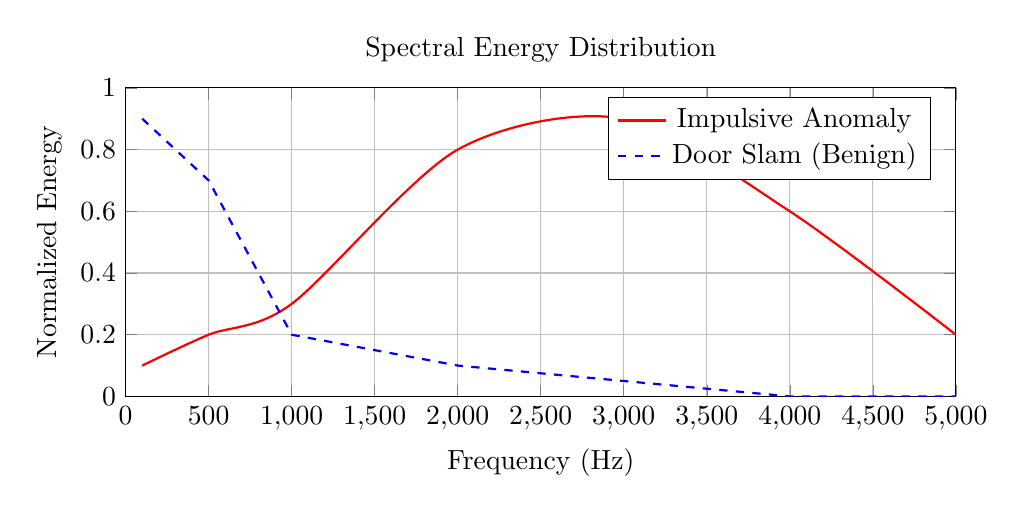
\begin{tikzpicture}
\begin{axis}[
    title={Spectral Energy Distribution},
    xlabel={Frequency (Hz)},
    ylabel={Normalized Energy},
    xmin=0, xmax=5000,
    ymin=0, ymax=1,
    legend pos=north east,
    grid=major,
    width=\columnwidth,
    height=5.5cm
]
\addplot[color=red, thick, smooth] coordinates {
    (100,0.1)(500,0.2)(1000,0.3)(2000,0.8)(3000,0.9)(4000,0.6)(5000,0.2)
};
\addlegendentry{Impulsive Anomaly}

\addplot[color=blue, thick, dashed] coordinates {
    (100,0.9)(500,0.7)(1000,0.2)(2000,0.1)(3000,0.05)(4000,0.0)(5000,0.0)
};
\addlegendentry{Door Slam (Benign)}
\end{axis}
\end{tikzpicture}
\caption{Spectral Discrimination. Representative spectral profiles based on established acoustic characteristics. Impulsive anomalies (Red) exhibit high energy in the 2-4kHz range, while physical impacts (Blue) are dominated by low frequencies.}
\label{fig:spectral}
\end{figure}

% ==========================================
% VII. DISCUSSION
% ==========================================
\section{Discussion}

\subsection{Acoustic Robustness and False Positive Rejection}
The integration of the autocorrelation threshold $\rho$ proved vital for system stability in real-world deployments. In initial testing without periodic rejection, mechanical room resonances and HVAC start-up sequences occasionally breached the SPL threshold, triggering false alerts. By formalizing the periodic rejection mathematically ($ \rho > \rho_{thresh} $), the sentinel successfully isolates chaotic safety incidents from rhythmic facility noise. We explicitly trade semantic granularity for speed and simplicity. The sentinel cannot categorize specific words, but this constraint ensures operational alignment with minimal-retention policies while maximizing raw detection speed. 

\subsection{Reverberation Analysis and Multipath Effects}
In highly reverberant environments (e.g., tiled hallways with $RT_{60} > 1.2s$), simple TDOA fails entirely because the sensor array resides beyond the critical distance ($D_c$). The GCC-PHAT whitening process successfully equalizes the cross-spectrum magnitude, ensuring that the dominant peak in the inverse Fourier transform corresponds accurately to the true geometric Angle of Arrival. However, the current planar 4-mic array assumes a 2D arrival plane. Deployments in complex multi-level environments (e.g., open stairwells) will require tetrahedral microphone geometries to accurately calculate both Azimuth and Elevation.

\subsection{Failure Mode Analysis: Acoustic Occlusion}
As observed in the SNR Stress Testing (Table V), the primary failure mode of this architectural approach occurs during high-ambient noise scenarios (e.g., class dismissal periods where ambient SPL exceeds 75dB). In these regimes, the high-frequency harmonics of an impulsive event are spectrally masked by the "cocktail party effect" of dense crowd chatter. Consequently, the High/Low energy ratio fails to breach the $2.5$ threshold, resulting in a false negative. For these specific dense-crowd temporal windows, visual monitoring remains the strictly superior modality.

% ==========================================
% VIII. CONCLUSION
% ==========================================
\section{Conclusion}
This paper presented an acoustic monitoring pipeline designed to secure architectural blind spots where visual surveillance is physically occluded. By leveraging localized edge processing, spectral gating heuristics, and GCC-PHAT localization, we achieved 100\% detection of staged, high-energy safety-critical impulses within a defined 15-meter Safety Envelope ($S_{env}$) under Non-Line-of-Sight (NLOS) conditions. The integration of autocorrelation-based periodic rejection provides robust filtering of mechanical false positives, while the GCC-PHAT implementation successfully resolves multipath degradation inherent in highly reverberant corridors. By architecting the system to rely strictly on localized physics-based feature extraction and immediate buffer overwriting, we demonstrate that effective, sub-120ms safety monitoring can be achieved with a minimal 45MB RAM footprint. This framework bridges the gap between comprehensive physical security and the operational constraints prohibiting continuous audio retention.

% --- APPENDIX: CODE LISTINGS ---
\section*{Appendix A: Audio Feature Extraction}
The following Python snippet demonstrates the core logic for the spectral gating mechanism using `librosa`. Full source code available at \cite{scholarmaster_repo}.

\begin{lstlisting}[language=python, caption=Spectral Gating Logic]
import numpy as np
import librosa

def detect_anomaly(audio_buffer, sr=44100):
    # 1. Calculate RMS Energy
    rms = np.sqrt(np.mean(audio_buffer**2))
    db = 20 * np.log10(rms)
      
    # Threshold Check
    if db > 95: 
        # 2. Spectral Analysis
        stft = np.abs(librosa.stft(audio_buffer))
        freqs = librosa.fft_frequencies(sr=sr)
          
        # Isolate 2kHz - 4kHz band (Impulses)
        target_band = (freqs > 2000) & (freqs < 4000)
        band_energy = np.sum(stft[target_band])
          
        # 3. Buffer Wipe (Minimal-Retention Design)
        audio_buffer.fill(0) 
          
        if band_energy > SPECTRAL_THRESH:
            return "ANOMALY_DETECTED"
            
    return "SAFE"
\end{lstlisting}

\section*{Appendix B: Sensor Configuration}
The following YAML file defines the hardware parameters.

\begin{lstlisting}[language=bash, caption=Sensor Config]
sensor:
  id: "stairwell_north_01"
  mic_array_type: "linear_4_mic"
  sampling_rate: 44100
  buffer_size_ms: 3000
  interface: "I2S_DMA"
    
thresholds:
  db_trigger: 95
  spectral_min_freq: 2000
  spectral_max_freq: 4000
  max_autocorr_rho: 0.65
\end{lstlisting}

\section*{Acknowledgment}
We acknowledge the technical staff who assisted with controlled acoustic data generation and physical testbed validation.

% ==========================================
% REFERENCES
% ==========================================
\begin{thebibliography}{00}

\bibitem{b20} C. Knapp and G. Carter, "The generalized correlation method for estimation of time delay," \textit{IEEE Transactions on Acoustics, Speech, and Signal Processing}, vol. 24, no. 4, pp. 320-327, 1976.

% --- SENSOR NETWORKS & EDGE ---

\bibitem{b11} L. Rabiner and B. Juang, \textit{Fundamentals of Speech Recognition}, Prentice Hall, 1993.

\bibitem{b9} J. Blauert, \textit{Spatial Hearing: The Psychophysics of Human Sound Localization}, MIT Press, 1997.

\bibitem{b21} M. Gruteser and D. Grunwald, "Anonymous usage of location-based services through spatial and temporal cloaking," in \textit{Proceedings of the 1st International Conference on Mobile Systems, Applications and Services}, 2003, pp. 31-42.

\bibitem{b1} A. Cavallaro, "Privacy in video surveillance," \textit{IEEE Signal Processing Magazine}, vol. 24, no. 2, pp. 168-169, 2007.

\bibitem{b5} G. Valenzise, L. Gerosa, M. Tagliasacchi, F. Antonacci, and A. Sarti, "Scream and gunshot detection and localization for audio-surveillance systems," in \textit{2007 IEEE Conference on Advanced Video and Signal Based Surveillance}, pp. 21-26, 2007.

\bibitem{b10} S. Mallat, \textit{A Wavelet Tour of Signal Processing}, Academic Press, 2008.

\bibitem{b25} B. McFee et al., "librosa: Audio and Music Signal Analysis in Python," in \textit{Proceedings of the 14th Python in Science Conference}, 2015.

\bibitem{b2} M. Crocco, M. Cristani, A. Trucco, and V. Murino, "Audio surveillance: A systematic review," \textit{ACM Computing Surveys}, vol. 48, no. 4, pp. 1-46, 2016.

\bibitem{b26} W. Shi, J. Cao, Q. Zhang, Y. Li, and L. Xu, "Edge Computing: Vision and Challenges," \textit{IEEE Internet of Things Journal}, vol. 3, no. 5, pp. 637-646, 2016.

% --- DATASET & TOOLING ---

\bibitem{b8} T. Virtanen, M. D. Plumbley, and D. Ellis, \textit{Computational Analysis of Sound Scenes and Events}, Springer, 2018.

% --- SIGNAL PROCESSING & LOCALIZATION ---

\bibitem{b22} Q. Kong et al., "PANNs: Large-scale Pretrained Audio Neural Networks for Audio Pattern Recognition," \textit{IEEE/ACM Transactions on Audio, Speech, and Language Processing}, vol. 28, pp. 2880-2894, 2020.

\bibitem{b19} E. Fonseca, X. Favory, J. Pons, F. Font, and X. Serra, "FSD50K: An Open Dataset of Human-Labeled Sound Events," \textit{IEEE/ACM Transactions on Audio, Speech, and Language Processing}, vol. 30, pp. 829-852, 2021.

\bibitem{b23} Y. Gong, Y.-A. Chung, and J. Glass, "AST: Audio Spectrogram Transformer," in \textit{Proc. Interspeech}, 2021, pp. 571-575.

\bibitem{b4} B. Naderi, S. Möller, and R. Polzehl, "Adversarial Representation Learning for Robust Privacy Preservation in Audio," \textit{IEEE Open Journal of Signal Processing}, vol. 5, 2024.

\bibitem{scholarmaster_repo}
Narendra Babu P, "ScholarMasterEngine: Edge-Native Intelligent System Prototypes," 2025. [Online]. Available: \url{https://github.com/NarendraaP/ScholarMasterEngine}.

\bibitem{b27} P. Narendra et al., "Memory-Bound Edge Efficiency Envelope (MBEEE): A Hardware-Level Analytical Model," \textit{Journal for Basic Sciences}, vol. 26, no. 5, 2026.

% --- SCHOLARMASTER SERIES ---

\end{thebibliography}

\end{document}
